\documentclass[twoside]{book}

% Packages required by doxygen
\usepackage{fixltx2e}
\usepackage{calc}
\usepackage{doxygen}
\usepackage{graphicx}
\usepackage[utf8]{inputenc}
\usepackage{makeidx}
\usepackage{multicol}
\usepackage{multirow}
\PassOptionsToPackage{warn}{textcomp}
\usepackage{textcomp}
\usepackage[nointegrals]{wasysym}
\usepackage[table]{xcolor}

% NLS support packages
\usepackage[spanish]{babel}
% Font selection
\usepackage[T1]{fontenc}
\usepackage{mathptmx}
\usepackage[scaled=.90]{helvet}
\usepackage{courier}
\usepackage{amssymb}
\usepackage{sectsty}
\renewcommand{\familydefault}{\sfdefault}
\allsectionsfont{%
  \fontseries{bc}\selectfont%
  \color{darkgray}%
}
\renewcommand{\DoxyLabelFont}{%
  \fontseries{bc}\selectfont%
  \color{darkgray}%
}
\newcommand{\+}{\discretionary{\mbox{\scriptsize$\hookleftarrow$}}{}{}}

% Page & text layout
\usepackage{geometry}
\geometry{%
  a4paper,%
  top=2.5cm,%
  bottom=2.5cm,%
  left=2.5cm,%
  right=2.5cm%
}
\tolerance=750
\hfuzz=15pt
\hbadness=750
\setlength{\emergencystretch}{15pt}
\setlength{\parindent}{0cm}
\setlength{\parskip}{0.2cm}
\makeatletter
\renewcommand{\paragraph}{%
  \@startsection{paragraph}{4}{0ex}{-1.0ex}{1.0ex}{%
    \normalfont\normalsize\bfseries\SS@parafont%
  }%
}
\renewcommand{\subparagraph}{%
  \@startsection{subparagraph}{5}{0ex}{-1.0ex}{1.0ex}{%
    \normalfont\normalsize\bfseries\SS@subparafont%
  }%
}
\makeatother

% Headers & footers
\usepackage{fancyhdr}
\pagestyle{fancyplain}
\fancyhead[LE]{\fancyplain{}{\bfseries\thepage}}
\fancyhead[CE]{\fancyplain{}{}}
\fancyhead[RE]{\fancyplain{}{\bfseries\leftmark}}
\fancyhead[LO]{\fancyplain{}{\bfseries\rightmark}}
\fancyhead[CO]{\fancyplain{}{}}
\fancyhead[RO]{\fancyplain{}{\bfseries\thepage}}
\fancyfoot[LE]{\fancyplain{}{}}
\fancyfoot[CE]{\fancyplain{}{}}
\fancyfoot[RE]{\fancyplain{}{\bfseries\scriptsize Generado el Miércoles, 19 de Noviembre de 2014 04\+:00\+:42 para C\+P\+P\+Unit\+Testing por Doxygen }}
\fancyfoot[LO]{\fancyplain{}{\bfseries\scriptsize Generado el Miércoles, 19 de Noviembre de 2014 04\+:00\+:42 para C\+P\+P\+Unit\+Testing por Doxygen }}
\fancyfoot[CO]{\fancyplain{}{}}
\fancyfoot[RO]{\fancyplain{}{}}
\renewcommand{\footrulewidth}{0.4pt}
\renewcommand{\chaptermark}[1]{%
  \markboth{#1}{}%
}
\renewcommand{\sectionmark}[1]{%
  \markright{\thesection\ #1}%
}

% Indices & bibliography
\usepackage{natbib}
\usepackage[titles]{tocloft}
\setcounter{tocdepth}{3}
\setcounter{secnumdepth}{5}
\makeindex

% Custom commands
\newcommand{\clearemptydoublepage}{%
  \newpage{\pagestyle{empty}\cleardoublepage}%
}


%===== C O N T E N T S =====

\begin{document}

% Titlepage & ToC
\pagenumbering{roman}
\begin{titlepage}
\vspace*{7cm}
\begin{center}%
{\Large C\+P\+P\+Unit\+Testing \\[1ex]\large 0.\+0.\+1 }\\
\vspace*{1cm}
{\large Generado por Doxygen 1.8.8}\\
\vspace*{0.5cm}
{\small Miércoles, 19 de Noviembre de 2014 04:00:42}\\
\end{center}
\end{titlepage}
\clearemptydoublepage
\tableofcontents
\clearemptydoublepage
\pagenumbering{arabic}

%--- Begin generated contents ---
\chapter{Indice jerárquico}
\section{Jerarquía de la clase}
Esta lista de herencias esta ordenada aproximadamente por orden alfabético\+:\begin{DoxyCompactList}
\item \contentsline{section}{Segunda}{\pageref{class_segunda}}{}
\item \contentsline{section}{T\+D\+D\+Prueba}{\pageref{class_t_d_d_prueba}}{}
\item Test\+Case\begin{DoxyCompactList}
\item \contentsline{section}{tddprueba\+\_\+spec}{\pageref{classtddprueba__spec}}{}
\end{DoxyCompactList}
\item Test\+Fixture\begin{DoxyCompactList}
\item \contentsline{section}{Segunda\+\_\+spec}{\pageref{class_segunda__spec}}{}
\end{DoxyCompactList}
\end{DoxyCompactList}

\chapter{Índice de clases}
\section{Class List}
Here are the classes, structs, unions and interfaces with brief descriptions\+:\begin{DoxyCompactList}
\item\contentsline{section}{{\bf Segunda} }{\pageref{class_segunda}}{}
\item\contentsline{section}{{\bf T\+D\+D\+Prueba} }{\pageref{class_t_d_d_prueba}}{}
\end{DoxyCompactList}

\chapter{Indice de archivos}
\section{Lista de archivos}
Lista de todos los archivos con descripciones breves\+:\begin{DoxyCompactList}
\item\contentsline{section}{lib/{\bf global\+Conf.\+h} \\*Archivo de configuración global del programa }{\pageref{global_conf_8h}}{}
\item\contentsline{section}{lib/{\bf main.\+cpp} \\*Ejemplo T\+D\+D para c++ }{\pageref{main_8cpp}}{}
\item\contentsline{section}{lib/tdd/{\bf segunda.\+cpp} }{\pageref{segunda_8cpp}}{}
\item\contentsline{section}{lib/tdd/{\bf segunda.\+h} }{\pageref{segunda_8h}}{}
\item\contentsline{section}{lib/tdd/{\bf tddprueba.\+cpp} }{\pageref{tddprueba_8cpp}}{}
\item\contentsline{section}{lib/tdd/{\bf tddprueba.\+h} }{\pageref{tddprueba_8h}}{}
\item\contentsline{section}{test/tdd/{\bf segunda\+\_\+spec.\+cpp} }{\pageref{segunda__spec_8cpp}}{}
\item\contentsline{section}{test/tdd/{\bf segunda\+\_\+spec.\+h} }{\pageref{segunda__spec_8h}}{}
\item\contentsline{section}{test/tdd/{\bf tddprueba\+\_\+spec.\+cpp} }{\pageref{tddprueba__spec_8cpp}}{}
\item\contentsline{section}{test/tdd/{\bf tddprueba\+\_\+spec.\+h} }{\pageref{tddprueba__spec_8h}}{}
\end{DoxyCompactList}

\chapter{Documentación de las clases}
\section{Segunda Class Reference}
\label{class_segunda}\index{Segunda@{Segunda}}


The documentation for this class was generated from the following files\+:\begin{DoxyCompactItemize}
\item 
lib/tdd/segunda.\+h\item 
lib/tdd/segunda.\+cpp\end{DoxyCompactItemize}

\section{Referencia de la Clase Segunda\+\_\+spec}
\label{class_segunda__spec}\index{Segunda\+\_\+spec@{Segunda\+\_\+spec}}


{\ttfamily \#include $<$segunda\+\_\+spec.\+h$>$}

Diagrama de herencias de Segunda\+\_\+spec\begin{figure}[H]
\begin{center}
\leavevmode
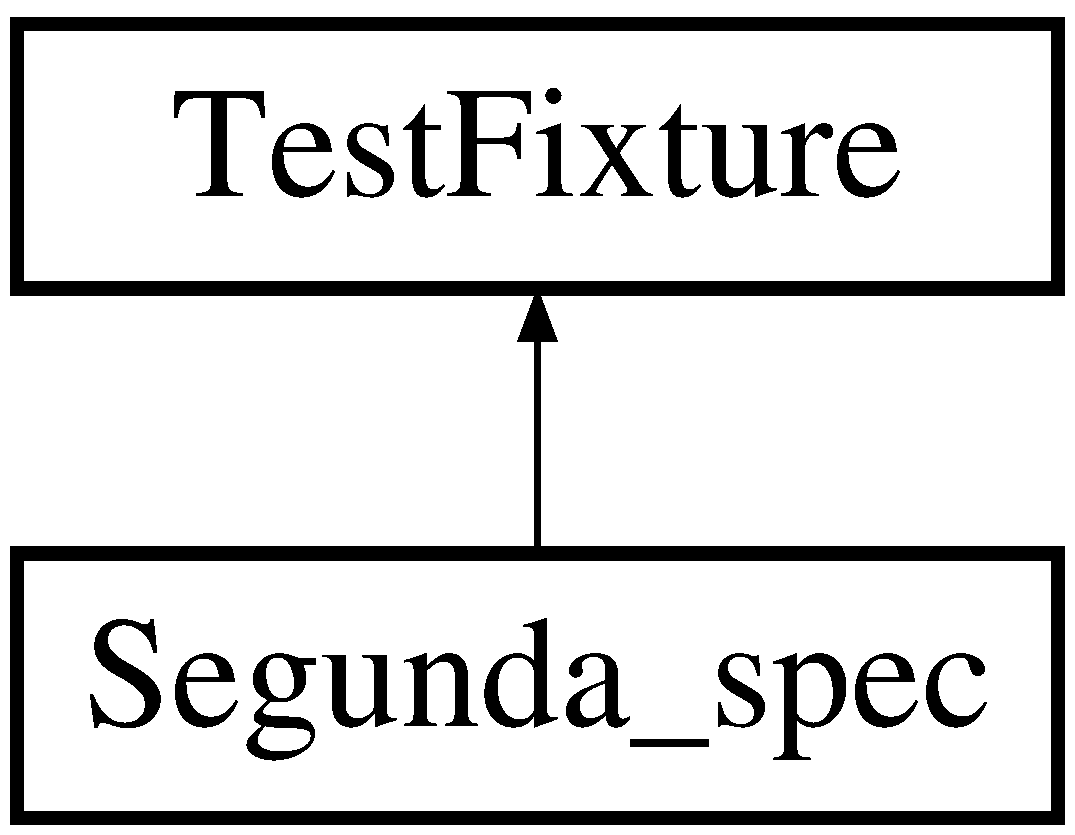
\includegraphics[height=2.000000cm]{class_segunda__spec}
\end{center}
\end{figure}
\subsection*{Métodos públicos}
\begin{DoxyCompactItemize}
\item 
{\bf Segunda\+\_\+spec} ()
\item 
void {\bf set\+Up} ()
\item 
void {\bf tear\+Down} ()
\end{DoxyCompactItemize}
\subsection*{Métodos públicos estáticos}
\begin{DoxyCompactItemize}
\item 
static Cpp\+Unit\+::\+Test $\ast$ {\bf suite} ()
\end{DoxyCompactItemize}
\subsection*{Métodos protegidos}
\begin{DoxyCompactItemize}
\item 
void {\bf test\+Sum} ()
\item 
void {\bf test\+Sub} ()
\end{DoxyCompactItemize}


\subsection{Descripción detallada}


Definición en la línea 11 del archivo segunda\+\_\+spec.\+h.



\subsection{Documentación del constructor y destructor}
\index{Segunda\+\_\+spec@{Segunda\+\_\+spec}!Segunda\+\_\+spec@{Segunda\+\_\+spec}}
\index{Segunda\+\_\+spec@{Segunda\+\_\+spec}!Segunda\+\_\+spec@{Segunda\+\_\+spec}}
\subsubsection[{Segunda\+\_\+spec}]{\setlength{\rightskip}{0pt plus 5cm}Segunda\+\_\+spec\+::\+Segunda\+\_\+spec (
\begin{DoxyParamCaption}
{}
\end{DoxyParamCaption}
)}\label{class_segunda__spec_ac98eba427182107b82e09941eada9ea4}


Definición en la línea 3 del archivo segunda\+\_\+spec.\+cpp.


\begin{DoxyCode}
3                            \{
4 \}
\end{DoxyCode}


\subsection{Documentación de las funciones miembro}
\index{Segunda\+\_\+spec@{Segunda\+\_\+spec}!set\+Up@{set\+Up}}
\index{set\+Up@{set\+Up}!Segunda\+\_\+spec@{Segunda\+\_\+spec}}
\subsubsection[{set\+Up}]{\setlength{\rightskip}{0pt plus 5cm}void Segunda\+\_\+spec\+::set\+Up (
\begin{DoxyParamCaption}
{}
\end{DoxyParamCaption}
)\hspace{0.3cm}{\ttfamily [inline]}}\label{class_segunda__spec_a6809b266524673161b7d8bb7c3f668df}


Definición en la línea 17 del archivo segunda\+\_\+spec.\+h.


\begin{DoxyCode}
17 \{\}
\end{DoxyCode}
\index{Segunda\+\_\+spec@{Segunda\+\_\+spec}!suite@{suite}}
\index{suite@{suite}!Segunda\+\_\+spec@{Segunda\+\_\+spec}}
\subsubsection[{suite}]{\setlength{\rightskip}{0pt plus 5cm}Cpp\+Unit\+::\+Test $\ast$ Segunda\+\_\+spec\+::suite (
\begin{DoxyParamCaption}
{}
\end{DoxyParamCaption}
)\hspace{0.3cm}{\ttfamily [static]}}\label{class_segunda__spec_afce85800fe161d9439d0d581a0777bff}


Definición en la línea 6 del archivo segunda\+\_\+spec.\+cpp.


\begin{DoxyCode}
6                                  \{
7    CppUnit::TestSuite *suiteOfTests = \textcolor{keyword}{new} CppUnit::TestSuite( \textcolor{stringliteral}{"CalculatorTestSuite"} );
8 
9 
10    suiteOfTests->addTest( \textcolor{keyword}{new} CppUnit::TestCaller<Segunda\_spec>(
11                                   \textcolor{stringliteral}{"Test Sum"},
12                                   &Segunda_spec::testSum ) );
13    suiteOfTests->addTest( \textcolor{keyword}{new} CppUnit::TestCaller<Segunda\_spec>(
14                                   \textcolor{stringliteral}{"Test Subtraction"},
15                                   &Segunda_spec::testSub ) );
16    \textcolor{keywordflow}{return} suiteOfTests;
17  \}
\end{DoxyCode}
\index{Segunda\+\_\+spec@{Segunda\+\_\+spec}!tear\+Down@{tear\+Down}}
\index{tear\+Down@{tear\+Down}!Segunda\+\_\+spec@{Segunda\+\_\+spec}}
\subsubsection[{tear\+Down}]{\setlength{\rightskip}{0pt plus 5cm}void Segunda\+\_\+spec\+::tear\+Down (
\begin{DoxyParamCaption}
{}
\end{DoxyParamCaption}
)\hspace{0.3cm}{\ttfamily [inline]}}\label{class_segunda__spec_a74e293686493cff3969b932ef0d7bcd5}


Definición en la línea 18 del archivo segunda\+\_\+spec.\+h.


\begin{DoxyCode}
18 \{\}
\end{DoxyCode}
\index{Segunda\+\_\+spec@{Segunda\+\_\+spec}!test\+Sub@{test\+Sub}}
\index{test\+Sub@{test\+Sub}!Segunda\+\_\+spec@{Segunda\+\_\+spec}}
\subsubsection[{test\+Sub}]{\setlength{\rightskip}{0pt plus 5cm}void Segunda\+\_\+spec\+::test\+Sub (
\begin{DoxyParamCaption}
{}
\end{DoxyParamCaption}
)\hspace{0.3cm}{\ttfamily [inline]}, {\ttfamily [protected]}}\label{class_segunda__spec_a8eb1777aaf44f467947ee295fe0d871e}


Definición en la línea 24 del archivo segunda\+\_\+spec.\+h.


\begin{DoxyCode}
24                      \{
25          CPPUNIT\_ASSERT(\textcolor{keyword}{true});
26       \}
\end{DoxyCode}
\index{Segunda\+\_\+spec@{Segunda\+\_\+spec}!test\+Sum@{test\+Sum}}
\index{test\+Sum@{test\+Sum}!Segunda\+\_\+spec@{Segunda\+\_\+spec}}
\subsubsection[{test\+Sum}]{\setlength{\rightskip}{0pt plus 5cm}void Segunda\+\_\+spec\+::test\+Sum (
\begin{DoxyParamCaption}
{}
\end{DoxyParamCaption}
)\hspace{0.3cm}{\ttfamily [inline]}, {\ttfamily [protected]}}\label{class_segunda__spec_a5a79448f5634fbb8daf600aaa5748751}


Definición en la línea 21 del archivo segunda\+\_\+spec.\+h.


\begin{DoxyCode}
21                      \{
22          CPPUNIT\_ASSERT(\textcolor{keyword}{true});
23       \}
\end{DoxyCode}


La documentación para esta clase fue generada a partir de los siguientes ficheros\+:\begin{DoxyCompactItemize}
\item 
test/tdd/{\bf segunda\+\_\+spec.\+h}\item 
test/tdd/{\bf segunda\+\_\+spec.\+cpp}\end{DoxyCompactItemize}

\section{Referencia de la Clase T\+D\+D\+Prueba}
\label{class_t_d_d_prueba}\index{T\+D\+D\+Prueba@{T\+D\+D\+Prueba}}


{\ttfamily \#include $<$tddprueba.\+h$>$}

\subsection*{Métodos públicos}
\begin{DoxyCompactItemize}
\item 
{\bf T\+D\+D\+Prueba} ()
\item 
int {\bf get\+Ultimo} ()
\end{DoxyCompactItemize}


\subsection{Descripción detallada}


Definición en la línea 19 del archivo tddprueba.\+h.



\subsection{Documentación del constructor y destructor}
\index{T\+D\+D\+Prueba@{T\+D\+D\+Prueba}!T\+D\+D\+Prueba@{T\+D\+D\+Prueba}}
\index{T\+D\+D\+Prueba@{T\+D\+D\+Prueba}!T\+D\+D\+Prueba@{T\+D\+D\+Prueba}}
\subsubsection[{T\+D\+D\+Prueba}]{\setlength{\rightskip}{0pt plus 5cm}T\+D\+D\+Prueba\+::\+T\+D\+D\+Prueba (
\begin{DoxyParamCaption}
{}
\end{DoxyParamCaption}
)}\label{class_t_d_d_prueba_a8ff2aa28eff38fde8ba23ebecc18c455}


Definición en la línea 14 del archivo tddprueba.\+cpp.


\begin{DoxyCode}
14 \{\}
\end{DoxyCode}


\subsection{Documentación de las funciones miembro}
\index{T\+D\+D\+Prueba@{T\+D\+D\+Prueba}!get\+Ultimo@{get\+Ultimo}}
\index{get\+Ultimo@{get\+Ultimo}!T\+D\+D\+Prueba@{T\+D\+D\+Prueba}}
\subsubsection[{get\+Ultimo}]{\setlength{\rightskip}{0pt plus 5cm}int T\+D\+D\+Prueba\+::get\+Ultimo (
\begin{DoxyParamCaption}
{}
\end{DoxyParamCaption}
)\hspace{0.3cm}{\ttfamily [inline]}}\label{class_t_d_d_prueba_aaa2c3c0342544285627f6b70468f8407}


Definición en la línea 22 del archivo tddprueba.\+h.


\begin{DoxyCode}
22 \{ \textcolor{keywordflow}{return} ultimoRes; \}
\end{DoxyCode}


La documentación para esta clase fue generada a partir de los siguientes ficheros\+:\begin{DoxyCompactItemize}
\item 
lib/tdd/{\bf tddprueba.\+h}\item 
lib/tdd/{\bf tddprueba.\+cpp}\end{DoxyCompactItemize}

\section{Referencia de la Clase tddprueba\+\_\+spec}
\label{classtddprueba__spec}\index{tddprueba\+\_\+spec@{tddprueba\+\_\+spec}}


{\ttfamily \#include $<$tddprueba\+\_\+spec.\+h$>$}

Diagrama de herencias de tddprueba\+\_\+spec\begin{figure}[H]
\begin{center}
\leavevmode
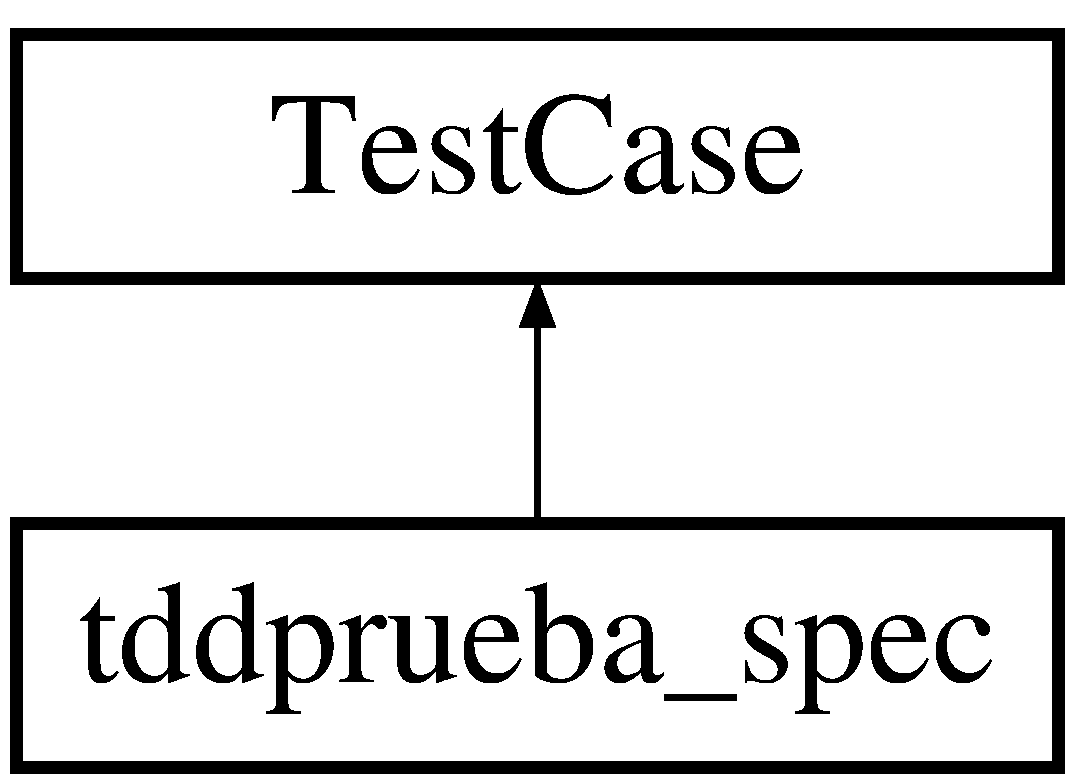
\includegraphics[height=2.000000cm]{classtddprueba__spec}
\end{center}
\end{figure}
\subsection*{Métodos públicos}
\begin{DoxyCompactItemize}
\item 
{\bf tddprueba\+\_\+spec} ()
\end{DoxyCompactItemize}


\subsection{Descripción detallada}


Definición en la línea 18 del archivo tddprueba\+\_\+spec.\+h.



\subsection{Documentación del constructor y destructor}
\index{tddprueba\+\_\+spec@{tddprueba\+\_\+spec}!tddprueba\+\_\+spec@{tddprueba\+\_\+spec}}
\index{tddprueba\+\_\+spec@{tddprueba\+\_\+spec}!tddprueba\+\_\+spec@{tddprueba\+\_\+spec}}
\subsubsection[{tddprueba\+\_\+spec}]{\setlength{\rightskip}{0pt plus 5cm}tddprueba\+\_\+spec\+::tddprueba\+\_\+spec (
\begin{DoxyParamCaption}
{}
\end{DoxyParamCaption}
)}\label{classtddprueba__spec_a543469c700658fa295a614f7c6923057}


Definición en la línea 14 del archivo tddprueba\+\_\+spec.\+cpp.


\begin{DoxyCode}
14 \{\}
\end{DoxyCode}


La documentación para esta clase fue generada a partir de los siguientes ficheros\+:\begin{DoxyCompactItemize}
\item 
test/tdd/{\bf tddprueba\+\_\+spec.\+h}\item 
test/tdd/{\bf tddprueba\+\_\+spec.\+cpp}\end{DoxyCompactItemize}

\chapter{Documentación de archivos}
\section{Referencia del Archivo lib/global\+Conf.h}
\label{global_conf_8h}\index{lib/global\+Conf.\+h@{lib/global\+Conf.\+h}}


Archivo de configuración global del programa.  


\subsection*{'defines'}
\begin{DoxyCompactItemize}
\item 
\#define {\bf T\+E\+S\+T\+\_\+\+C\+H\+E\+C\+K\+I\+N\+G}~true
\end{DoxyCompactItemize}


\subsection{Descripción detallada}
Archivo de configuración global del programa. 

\begin{DoxyAuthor}{Autor}
Wyllman {\tt wyllman@gmail.\+com} 
\end{DoxyAuthor}
\begin{DoxyVersion}{Versión}
0.\+0.\+1 
\end{DoxyVersion}
\begin{DoxyDate}{Fecha}
Noviembre, 2014 
\end{DoxyDate}
\subsection{D\+E\+S\+C\+R\+I\+P\+T\+I\+O\+N}\label{main_8cpp_DESCRIPTION}
Archivo de configuración global del programa. Este archivo contiene\+:
\begin{DoxyItemize}
\item Directivas de preprocesamiento para el compilador. En este caso, comprobar si se va a compilar o no el código para pasar los test. (T\+E\+S\+T\+\_\+\+C\+H\+E\+C\+K\+I\+N\+G) 
\end{DoxyItemize}

Definición en el archivo {\bf global\+Conf.\+h}.



\subsection{Documentación de los 'defines'}
\index{global\+Conf.\+h@{global\+Conf.\+h}!T\+E\+S\+T\+\_\+\+C\+H\+E\+C\+K\+I\+N\+G@{T\+E\+S\+T\+\_\+\+C\+H\+E\+C\+K\+I\+N\+G}}
\index{T\+E\+S\+T\+\_\+\+C\+H\+E\+C\+K\+I\+N\+G@{T\+E\+S\+T\+\_\+\+C\+H\+E\+C\+K\+I\+N\+G}!global\+Conf.\+h@{global\+Conf.\+h}}
\subsubsection[{T\+E\+S\+T\+\_\+\+C\+H\+E\+C\+K\+I\+N\+G}]{\setlength{\rightskip}{0pt plus 5cm}\#define T\+E\+S\+T\+\_\+\+C\+H\+E\+C\+K\+I\+N\+G~true}\label{global_conf_8h_a1adf200feffe9d395e8cf3acd3d029d8}
Se define la macro T\+E\+S\+T\+\_\+\+C\+H\+E\+C\+K\+I\+N\+G para controlar el uso de cppunit (T\+D\+D) a nivel de compilación.

Poner a false para desactivar las pruebas unitarias. 

Definición en la línea 27 del archivo global\+Conf.\+h.


\section{Referencia del Archivo lib/main.cpp}
\label{main_8cpp}\index{lib/main.\+cpp@{lib/main.\+cpp}}


Ejemplo T\+D\+D para c++.  


{\ttfamily \#include \char`\"{}global\+Conf.\+h\char`\"{}}\\*
{\ttfamily \#include $<$iostream$>$}\\*
\subsection*{Funciones}
\begin{DoxyCompactItemize}
\item 
int {\bf main} (int argc, char $\ast$argv[$\,$])
\begin{DoxyCompactList}\small\item\em main \end{DoxyCompactList}\end{DoxyCompactItemize}


\subsection{Descripción detallada}
Ejemplo T\+D\+D para c++. 

\begin{DoxyAuthor}{Autor}
Wyllman {\tt wyllman@gmail.\+com} 
\end{DoxyAuthor}
\begin{DoxyVersion}{Versión}
0.\+0.\+1 
\end{DoxyVersion}
\begin{DoxyDate}{Fecha}
Noviembre, 2014 
\end{DoxyDate}
\subsection{D\+E\+S\+C\+R\+I\+P\+T\+I\+O\+N}\label{main_8cpp_DESCRIPTION}
Programa de ejemplo en c++ para el uso de la metodología T\+D\+D, usando las librerías Cpp\+Unit.

Archivo principal de ejecución, encargado de ejecutar las pruebas (según la configuración del archivo \doxyref{global\+Conf.\+h}{p.}{global_conf_8h})

Las librerías Cpp\+Unit descargadas de\+: \begin{DoxySeeAlso}{Ver también}
{\tt http\+://sourceforge.\+net/projects/cppunit/} 
\end{DoxySeeAlso}


Definición en el archivo {\bf main.\+cpp}.



\subsection{Documentación de las funciones}
\index{main.\+cpp@{main.\+cpp}!main@{main}}
\index{main@{main}!main.\+cpp@{main.\+cpp}}
\subsubsection[{main}]{\setlength{\rightskip}{0pt plus 5cm}int main (
\begin{DoxyParamCaption}
\item[{int}]{argc, }
\item[{char $\ast$}]{argv[$\,$]}
\end{DoxyParamCaption}
)}\label{main_8cpp_a0ddf1224851353fc92bfbff6f499fa97}


main 


\begin{DoxyParams}{Parámetros}
{\em argc} & \\
\hline
{\em argv} & \\
\hline
\end{DoxyParams}
\begin{DoxyReturn}{Devuelve}

\end{DoxyReturn}


Definición en la línea 42 del archivo main.\+cpp.


\begin{DoxyCode}
42                                  \{
43     cout << \textcolor{stringliteral}{"Iniciando el ejemplo de TDD..."} << endl;
44 
45 \textcolor{preprocessor}{#if TEST\_CHECKING}
46     cout << \textcolor{stringliteral}{"Modo testeo activado."} << endl;
47     cout << \textcolor{stringliteral}{"Iniciando test..."} << endl;
48 
49     CppUnit::TextUi::TestRunner runner; \textcolor{comment}{/*** Crear el objeto de CppUnit que ejecutará las pruebas */}
50     runner.addTest(\textcolor{keyword}{new} tddprueba_spec ());
51     runner.addTest(Segunda_spec::suite());
52     runner.run();
53 \textcolor{preprocessor}{#else}
54    cout << \textcolor{stringliteral}{"Sin modo testeo."} << endl;
55 \textcolor{preprocessor}{#endif}
56 
57    cout << \textcolor{stringliteral}{"Finalizando el ejemplo de TDD..."} << endl;
58     \textcolor{keywordflow}{return} 0;
59 \}
\end{DoxyCode}

\section{Referencia del Archivo lib/tdd/segunda.cpp}
\label{segunda_8cpp}\index{lib/tdd/segunda.\+cpp@{lib/tdd/segunda.\+cpp}}
{\ttfamily \#include \char`\"{}lib/tdd/segunda.\+h\char`\"{}}\\*


\subsection{Descripción detallada}
\begin{DoxyAuthor}{Autor}
Wyllman {\tt wyllman@gmail.\+com} 
\end{DoxyAuthor}
\begin{DoxyVersion}{Versión}
0.\+0.\+1 
\end{DoxyVersion}
\begin{DoxyDate}{Fecha}
Noviembre, 2014 
\end{DoxyDate}
\subsection{D\+E\+S\+C\+R\+I\+P\+T\+I\+O\+N}\label{main_8cpp_DESCRIPTION}


Definición en el archivo {\bf segunda.\+cpp}.


\section{Referencia del Archivo lib/tdd/segunda.h}
\label{segunda_8h}\index{lib/tdd/segunda.\+h@{lib/tdd/segunda.\+h}}
\subsection*{Clases}
\begin{DoxyCompactItemize}
\item 
class {\bf Segunda}
\end{DoxyCompactItemize}


\subsection{Descripción detallada}
\begin{DoxyAuthor}{Autor}
Wyllman {\tt wyllman@gmail.\+com} 
\end{DoxyAuthor}
\begin{DoxyVersion}{Versión}
0.\+0.\+1 
\end{DoxyVersion}
\begin{DoxyDate}{Fecha}
Noviembre, 2014 
\end{DoxyDate}
\subsection{D\+E\+S\+C\+R\+I\+P\+T\+I\+O\+N}\label{main_8cpp_DESCRIPTION}


Definición en el archivo {\bf segunda.\+h}.


\section{Referencia del Archivo lib/tdd/tddprueba.cpp}
\label{tddprueba_8cpp}\index{lib/tdd/tddprueba.\+cpp@{lib/tdd/tddprueba.\+cpp}}
{\ttfamily \#include \char`\"{}lib/tdd/tddprueba.\+h\char`\"{}}\\*

\section{Referencia del Archivo lib/tdd/tddprueba.h}
\label{tddprueba_8h}\index{lib/tdd/tddprueba.\+h@{lib/tdd/tddprueba.\+h}}
\subsection*{Clases}
\begin{DoxyCompactItemize}
\item 
class {\bf T\+D\+D\+Prueba}
\end{DoxyCompactItemize}


\subsection{Descripción detallada}
\begin{DoxyAuthor}{Autor}
Wyllman {\tt wyllman@gmail.\+com} 
\end{DoxyAuthor}
\begin{DoxyVersion}{Versión}
0.\+0.\+1 
\end{DoxyVersion}
\begin{DoxyDate}{Fecha}
Noviembre, 2014 
\end{DoxyDate}
\subsection{D\+E\+S\+C\+R\+I\+P\+T\+I\+O\+N}\label{main_8cpp_DESCRIPTION}


Definición en el archivo {\bf tddprueba.\+h}.


\section{Referencia del Archivo test/tdd/segunda\+\_\+spec.cpp}
\label{segunda__spec_8cpp}\index{test/tdd/segunda\+\_\+spec.\+cpp@{test/tdd/segunda\+\_\+spec.\+cpp}}
{\ttfamily \#include \char`\"{}test/tdd/segunda\+\_\+spec.\+h\char`\"{}}\\*


\subsection{Descripción detallada}
\begin{DoxyAuthor}{Autor}
Wyllman {\tt wyllman@gmail.\+com} 
\end{DoxyAuthor}
\begin{DoxyVersion}{Versión}
0.\+0.\+1 
\end{DoxyVersion}
\begin{DoxyDate}{Fecha}
Noviembre, 2014 
\end{DoxyDate}
\subsection{D\+E\+S\+C\+R\+I\+P\+T\+I\+O\+N}\label{main_8cpp_DESCRIPTION}


Definición en el archivo {\bf segunda\+\_\+spec.\+cpp}.


\section{Referencia del Archivo test/tdd/segunda\+\_\+spec.h}
\label{segunda__spec_8h}\index{test/tdd/segunda\+\_\+spec.\+h@{test/tdd/segunda\+\_\+spec.\+h}}
{\ttfamily \#include $<$cppunit/\+Test\+Fixture.\+h$>$}\\*
{\ttfamily \#include $<$cppunit/\+Test\+Assert.\+h$>$}\\*
{\ttfamily \#include $<$cppunit/\+Test\+Caller.\+h$>$}\\*
{\ttfamily \#include $<$cppunit/\+Test\+Suite.\+h$>$}\\*
{\ttfamily \#include \char`\"{}../../lib/tdd/segunda.\+h\char`\"{}}\\*
\subsection*{Clases}
\begin{DoxyCompactItemize}
\item 
class {\bf Segunda\+\_\+spec}
\end{DoxyCompactItemize}

\section{Referencia del Archivo test/tdd/tddprueba\+\_\+spec.cpp}
\label{tddprueba__spec_8cpp}\index{test/tdd/tddprueba\+\_\+spec.\+cpp@{test/tdd/tddprueba\+\_\+spec.\+cpp}}
{\ttfamily \#include \char`\"{}test/tdd/tddprueba\+\_\+spec.\+h\char`\"{}}\\*

\section{Referencia del Archivo test/tdd/tddprueba\+\_\+spec.h}
\label{tddprueba__spec_8h}\index{test/tdd/tddprueba\+\_\+spec.\+h@{test/tdd/tddprueba\+\_\+spec.\+h}}
{\ttfamily \#include $<$cppunit/\+Test\+Case.\+h$>$}\\*
{\ttfamily \#include \char`\"{}../../lib/tdd/tddprueba.\+h\char`\"{}}\\*
\subsection*{Clases}
\begin{DoxyCompactItemize}
\item 
class {\bf tddprueba\+\_\+spec}
\end{DoxyCompactItemize}


\subsection{Descripción detallada}
\begin{DoxyAuthor}{Autor}
Wyllman {\tt wyllman@gmail.\+com} 
\end{DoxyAuthor}
\begin{DoxyVersion}{Versión}
0.\+0.\+1 
\end{DoxyVersion}
\begin{DoxyDate}{Fecha}
Noviembre, 2014 
\end{DoxyDate}
\subsection{D\+E\+S\+C\+R\+I\+P\+T\+I\+O\+N}\label{main_8cpp_DESCRIPTION}


Definición en el archivo {\bf tddprueba\+\_\+spec.\+h}.


%--- End generated contents ---

% Index
\newpage
\phantomsection
\addcontentsline{toc}{chapter}{Índice}
\printindex

\end{document}
